% ============================================================================
% Figure 1: Overall solver-family comparison (valid-solution rate & timeout rate)
% Compiles standalone with pdflatex; also \input-able inside a figure environment.
% Data source: paper/tables/table1_aggregate_comparison.csv (audited against
% data/results/benchmark_sat_vs_nonsat.csv and data/results/backtracking_results.csv).
% Denominators: SAT 760 attempted (80 predeclared exclusions removed);
% CP-SAT 120 attempted; Backtracking 120 attempted (0 exclusions).
% ============================================================================
\documentclass[border=5pt]{standalone}
\usepackage{pgfplots}
\pgfplotsset{compat=1.18}
\begin{document}
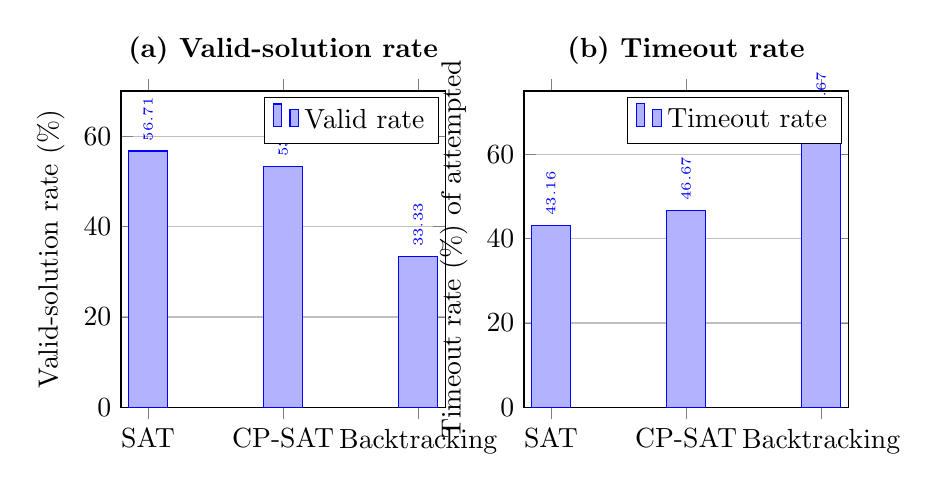
\begin{tikzpicture}
  % ---- Panel (a): valid-solution rate ----
  \begin{axis}[
    name=plotA,
    ybar, bar width=0.5cm, bar shift=0pt,
    symbolic x coords={SAT,CP-SAT,Backtracking},
    xtick=data,
    ylabel={Valid-solution rate (\%)},
    ymin=0, ymax=70,
    ymajorgrids=true,
    title style={font=\bfseries},
    title={(a) Valid-solution rate},
    width=0.47\textwidth, height=5.6cm,
    nodes near coords,
    nodes near coords align={vertical},
    every node near coord/.append style={font=\tiny\bfseries, rotate=90, anchor=west},
  ]
  \addplot coordinates {(SAT,56.71) (CP-SAT,53.33) (Backtracking,33.33)};
  \addlegendentry{Valid rate}
  \end{axis}

  % ---- Panel (b): timeout rate ----
  \begin{axis}[
    at={(plotA.east)}, anchor=west, xshift=1.0cm,
    ybar, bar width=0.5cm, bar shift=0pt,
    symbolic x coords={SAT,CP-SAT,Backtracking},
    xtick=data,
    ylabel={Timeout rate (\%) of attempted},
    ymin=0, ymax=75,
    ymajorgrids=true,
    title style={font=\bfseries},
    title={(b) Timeout rate},
    width=0.47\textwidth, height=5.6cm,
    nodes near coords,
    nodes near coords align={vertical},
    every node near coord/.append style={font=\tiny\bfseries, rotate=90, anchor=west},
  ]
  \addplot coordinates {(SAT,43.16) (CP-SAT,46.67) (Backtracking,66.67)};
  \addlegendentry{Timeout rate}
  \end{axis}
\end{tikzpicture}
\end{document}
